\begin{center}
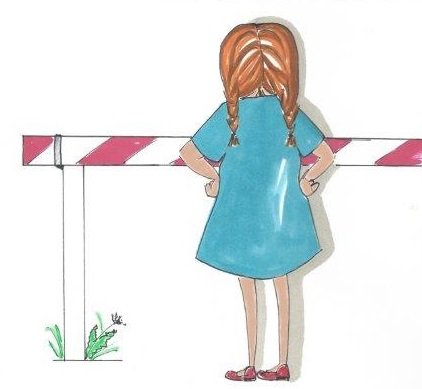
\includegraphics[width=0.4\textwidth]{content/3/chapter6/images/18.png}\\
Cippi在栅栏外等待
\end{center}

锁存器(门闩)和栅栏属于协调类型,可以阻塞线程,直到计数器变为零。C++20中有两种类型的门闩和栅栏:std::latch和std::barrier。并发调用std::latch或std::barrier的成员函数不会产生数据竞争。

首先,有两个问题:

\begin{enumerate}
\item 
这两种协调线程的机制之间有什么区别?std::latch只能使用一次,但std::barrier可以使用多次。std::latch在多线程管理一个任务时很有用,std::barrier可以帮助管理多个线程的重复任务。此外,std::barrier可在完成步骤中执行函数,这里的“完成步骤”指的是计数器变为零时的状态。

\item 
在C++11和C++14中用future、线程或条件变量与锁结合的情况下,门闩和栅栏支持哪些用例?门闩和栅栏没有解决新的用例,但是它们的使用要容易得多。因为它们经常在内部使用\href{https://en.wikipedia.org/wiki/Non-blocking_algorithm}{无锁}机制,所以性能会更好。
\end{enumerate}

\subsubsubsection{6.4.1\hspace{0.2cm}std::latch}

现在,来了解一下std::latch的接口。

\begin{table}[H]
\centering
\begin{tabular}{ll}
\textbf{成员函数} & \textbf{std::latch latat成员函数的描述}          \\ \hline
lat.count\_down(upd = 1)       & 按upd原子地递减计数器,而不阻塞调用者。  \\
lat.try\_wait()          & 若counter == 0则返回true。 \\
lat.wait()                     & 若counter == 0立即返回。若不阻塞,直到counter == 0再返回。 \\
lat.arrive\_and\_wait(upd = 1) &等价于count\_down(upd); wait();.                              
\end{tabular}
\end{table}

upd的默认值为1。当upd大于计数器或为负数时,行为未定义。使用lat.try\_wait()从不会真正等待,正如其名称一样。

下面的bossWorkers.cpp中,使用两个std::latch来构建一个boss-workers工作流。我使用synchronizedOut函数将输出同步到std::cout(第13行),使工作流更容易使用这种同步方式。

\begin{lstlisting}[style=styleCXX]
// bossWorkers.cpp

#include <iostream>
#include <mutex>
#include <latch>
#include <thread>

std::latch workDone(6);
std::latch goHome(1);

std::mutex coutMutex;

void synchronizedOut(const std::string& s) {
	std::lock_guard<std::mutex> lo(coutMutex);
	std::cout << s;
}

class Worker {
public:
	Worker(std::string n): name(n) { }
	
	void operator() (){
		// notify the boss when work is done
		synchronizedOut(name + ": " + "Work done!\n");
		workDone.count_down();
		
		// waiting before going home
		goHome.wait();
		synchronizedOut(name + ": " + "Good bye!\n");
	}
private:
	std::string name;
};

int main() {

	std::cout << '\n';
	
	std::cout << "BOSS: START WORKING! " << '\n';
	
	Worker herb(" Herb");
	std::thread herbWork(herb);
	
	Worker scott(" Scott");
	std::thread scottWork(scott);
	
	Worker bjarne(" Bjarne");
	std::thread bjarneWork(bjarne);
	
	Worker andrei(" Andrei");
	std::thread andreiWork(andrei);
	
	Worker andrew(" Andrew");
	std::thread andrewWork(andrew);
	
	Worker david(" David");
	std::thread davidWork(david);
	
	workDone.wait();
	
	std::cout << '\n';
	
	goHome.count_down();
	
	std::cout << "BOSS: GO HOME!" << '\n';
	
	herbWork.join();
	scottWork.join();
	bjarneWork.join();
	andreiWork.join();
	andrewWork.join();
	davidWork.join();

}
\end{lstlisting}

六个工人herb, scott, bjarne, andrei, andrew和david(第41 - 57行)必须完成他们的工作。当每个人都完成了他的工作时,开始倒数std::latch workDone(第25行)。boss(主线程)在第59行阻塞,直到计数器变为0。当计数器为0时,boss使用第二个std::latch goHome向其员工发出回家的信号。所以,初始计数器是1(第9行),goHome.wait()会阻塞直到计数器变为0。

\begin{center}
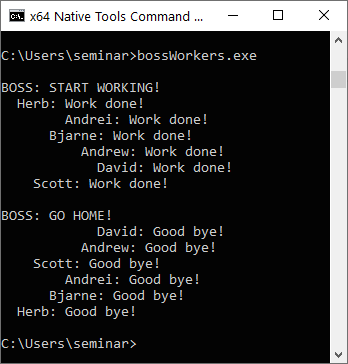
\includegraphics[width=0.55\textwidth]{content/3/chapter6/images/19.png}\\
\end{center}

研究这个工作流时,可能会注意到其可以在没有老板的情况下执行。

\begin{lstlisting}[style=styleCXX]
// workers.cpp

#include <iostream>
#include <barrier>
#include <mutex>
#include <thread>

std::latch workDone(6);
std::mutex coutMutex;

void synchronizedOut(const std::string& s) {
	std::lock_guard<std::mutex> lo(coutMutex);
	std::cout << s;
}

class Worker {
public:
	Worker(std::string n): name(n) { }

	void operator() () {
		synchronizedOut(name + ": " + "Work done!\n");
		workDone.arrive_and_wait(); // wait until all work is done
		synchronizedOut(name + ": " + "See you tomorrow!\n");
	}
private:
	std::string name;
};

int main() {

	std::cout << '\n';
	
	Worker herb(" Herb");
	std::thread herbWork(herb);
	
	Worker scott(" Scott");
	std::thread scottWork(scott);
	
	Worker bjarne(" Bjarne");
	std::thread bjarneWork(bjarne);
	
	Worker andrei(" Andrei");
	std::thread andreiWork(andrei);
	
	Worker andrew(" Andrew");
	std::thread andrewWork(andrew);
	
	Worker david(" David");
	std::thread davidWork(david);
	
	herbWork.join();
	scottWork.join();
	bjarneWork.join();
	andreiWork.join();
	andrewWork.join();
	davidWork.join();

}
\end{lstlisting}

这个简化的工作流程中,不需要添加太多的内容。wordDone.arrival\_and\_wait()(第22行)等价于count\_down(upd);wait();。所以,工人间可以相互协调,不再需要老板,就和bossWorkers.cpp一样。

\begin{center}
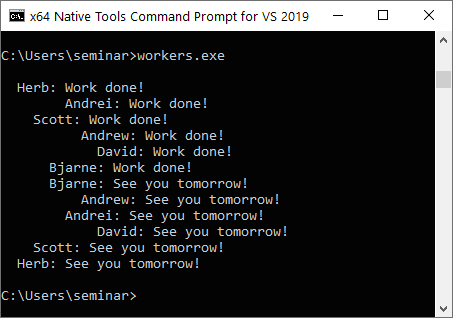
\includegraphics[width=0.6\textwidth]{content/3/chapter6/images/20.png}\\
\end{center}

std::barrier与std::latch类似。

\subsubsubsection{6.4.2\hspace{0.2cm}std::barrier}

std::latch和std::barrier之间有两个区别。首先,可以多次使用std::barrier;其次,可以为下一步(迭代)设置计数器。计数器变为零之后,“完成步骤”立即开始。“完成步骤”中,调用一个可调用对象。std::barrier在它的构造函数中,可以获得这个可调用的对象。

“完成步骤”执行以下操作:

\begin{enumerate}
\item 
阻塞所有线程。

\item 
任意线程解除阻塞并执行可调用对象。

\item 
若完成了“完成步骤”,则所有线程都将解除阻塞。
\end{enumerate}

\begin{table}[H]
\centering
\begin{tabular}{ll}
\textbf{成员函数}         & \textbf{std::barrier bar成员函数的描述}                                   \\ \hline
bar.arrive(upd)         & 按upd自动递减计数器。         \\
bar.wait()              & 在同步点上阻塞,直到完成步骤完成。  \\
bar.arrive\_and\_wait() & 等价于wait(arrive())                  \\
bar.arrive\_and\_drop() & 将当前阶段和后续阶段的计数器减1。 \\
std::barrier::max       & 获取实现支持的最大值。
\end{tabular}
\end{table}

bar.arrival\_and\_drop()会让计数器在下一阶段减1,fullTimePartTimeWorkers.cpp将第二阶段的工作人员数量减半。

\hspace*{\fill} \\ %插入空行
\noindent
\textbf{全职和兼职员工}
\begin{lstlisting}[style=styleCXX]
// fullTimePartTimeWorkers.cpp

#include <iostream>
#include <barrier>
#include <mutex>
#include <string>
#include <thread>

std::barrier workDone(6);
std::mutex coutMutex;

void synchronizedOut(const std::string& s) {
	std::lock_guard<std::mutex> lo(coutMutex);
	std::cout << s;
}

class FullTimeWorker {
public:
	FullTimeWorker(std::string n): name(n) { }
	
	void operator() () {
		synchronizedOut(name + ": " + "Morning work done!\n");
		workDone.arrive_and_wait(); // Wait until morning work is done
		synchronizedOut(name + ": " + "Afternoon work done!\n");
		workDone.arrive_and_wait(); // Wait until afternoon work is done

	}
private:
	std::string name;
};

class PartTimeWorker {
public:
	PartTimeWorker(std::string n): name(n) { }

	void operator() () {
		synchronizedOut(name + ": " + "Morning work done!\n");
		workDone.arrive_and_drop(); // Wait until morning work is done
	}
private:
	std::string name;
};

int main() {

	std::cout << '\n';
	
	FullTimeWorker herb(" Herb");
	std::thread herbWork(herb);
	
	FullTimeWorker scott(" Scott");
	std::thread scottWork(scott);
	
	FullTimeWorker bjarne(" Bjarne");
	std::thread bjarneWork(bjarne);
	PartTimeWorker andrei(" Andrei");
	std::thread andreiWork(andrei);
	
	PartTimeWorker andrew(" Andrew");
	std::thread andrewWork(andrew);
	
	PartTimeWorker david(" David");
	std::thread davidWork(david);
	
	herbWork.join();
	scottWork.join();
	bjarneWork.join();
	andreiWork.join();
	andrewWork.join();
	davidWork.join();

}
\end{lstlisting}

这个工作流由两种工人组成:全职工人(第17行)和兼职工人(第32行)。兼职工人在上午工作,全职工人在上午和下午工作,所以全职工作人员使用workDone.arrive\_and\_wait()两次(第23行和第25行),而兼职工作者只使用workDone.arrive\_and\_drop()(第38行)一次。workDone.arrive\_and\_drop()会让兼职工作者跳过下午的工作。相应地,计数器在第一阶段(上午)的值为6,在第二阶段(下午)的值会变为3。

\begin{center}
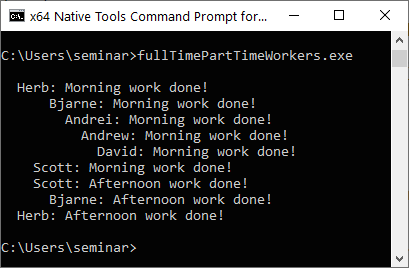
\includegraphics[width=0.6\textwidth]{content/3/chapter6/images/21.png}\\
全职和兼职工作者
\end{center}

\begin{tcolorbox}[breakable,enhanced jigsaw,colback=mygreen!5!white,colframe=mygreen!75!black,title={总结}]
	
\begin{itemize}
\item 
门闩和栅栏都是协调类型,可以阻塞线程,直到计数器变为零。std::latch只能使用一次,而std::barrier可以使用多次。

\item 
std::latch多用于多线程管理一次性任务,std::barrier多用于多线程管理重复的任务。
\end{itemize}
	
\end{tcolorbox}

\newpage














